\section{Simulation Results}
Figures \ref{simFig1}, \ref{simFig2} and \ref{simFig3} show the comparison of the bounds obtained via our novel method to bounds obtained using the transfer function method as well as simulation results. For each RSC code, the codeword is BPSK modulated and transmitted over the AWGN channel. At the receiver end, the Viterbi Algorithm is used to decode before a decision is made on the decoded sequence.

\begin{figure}[h]
\centering
		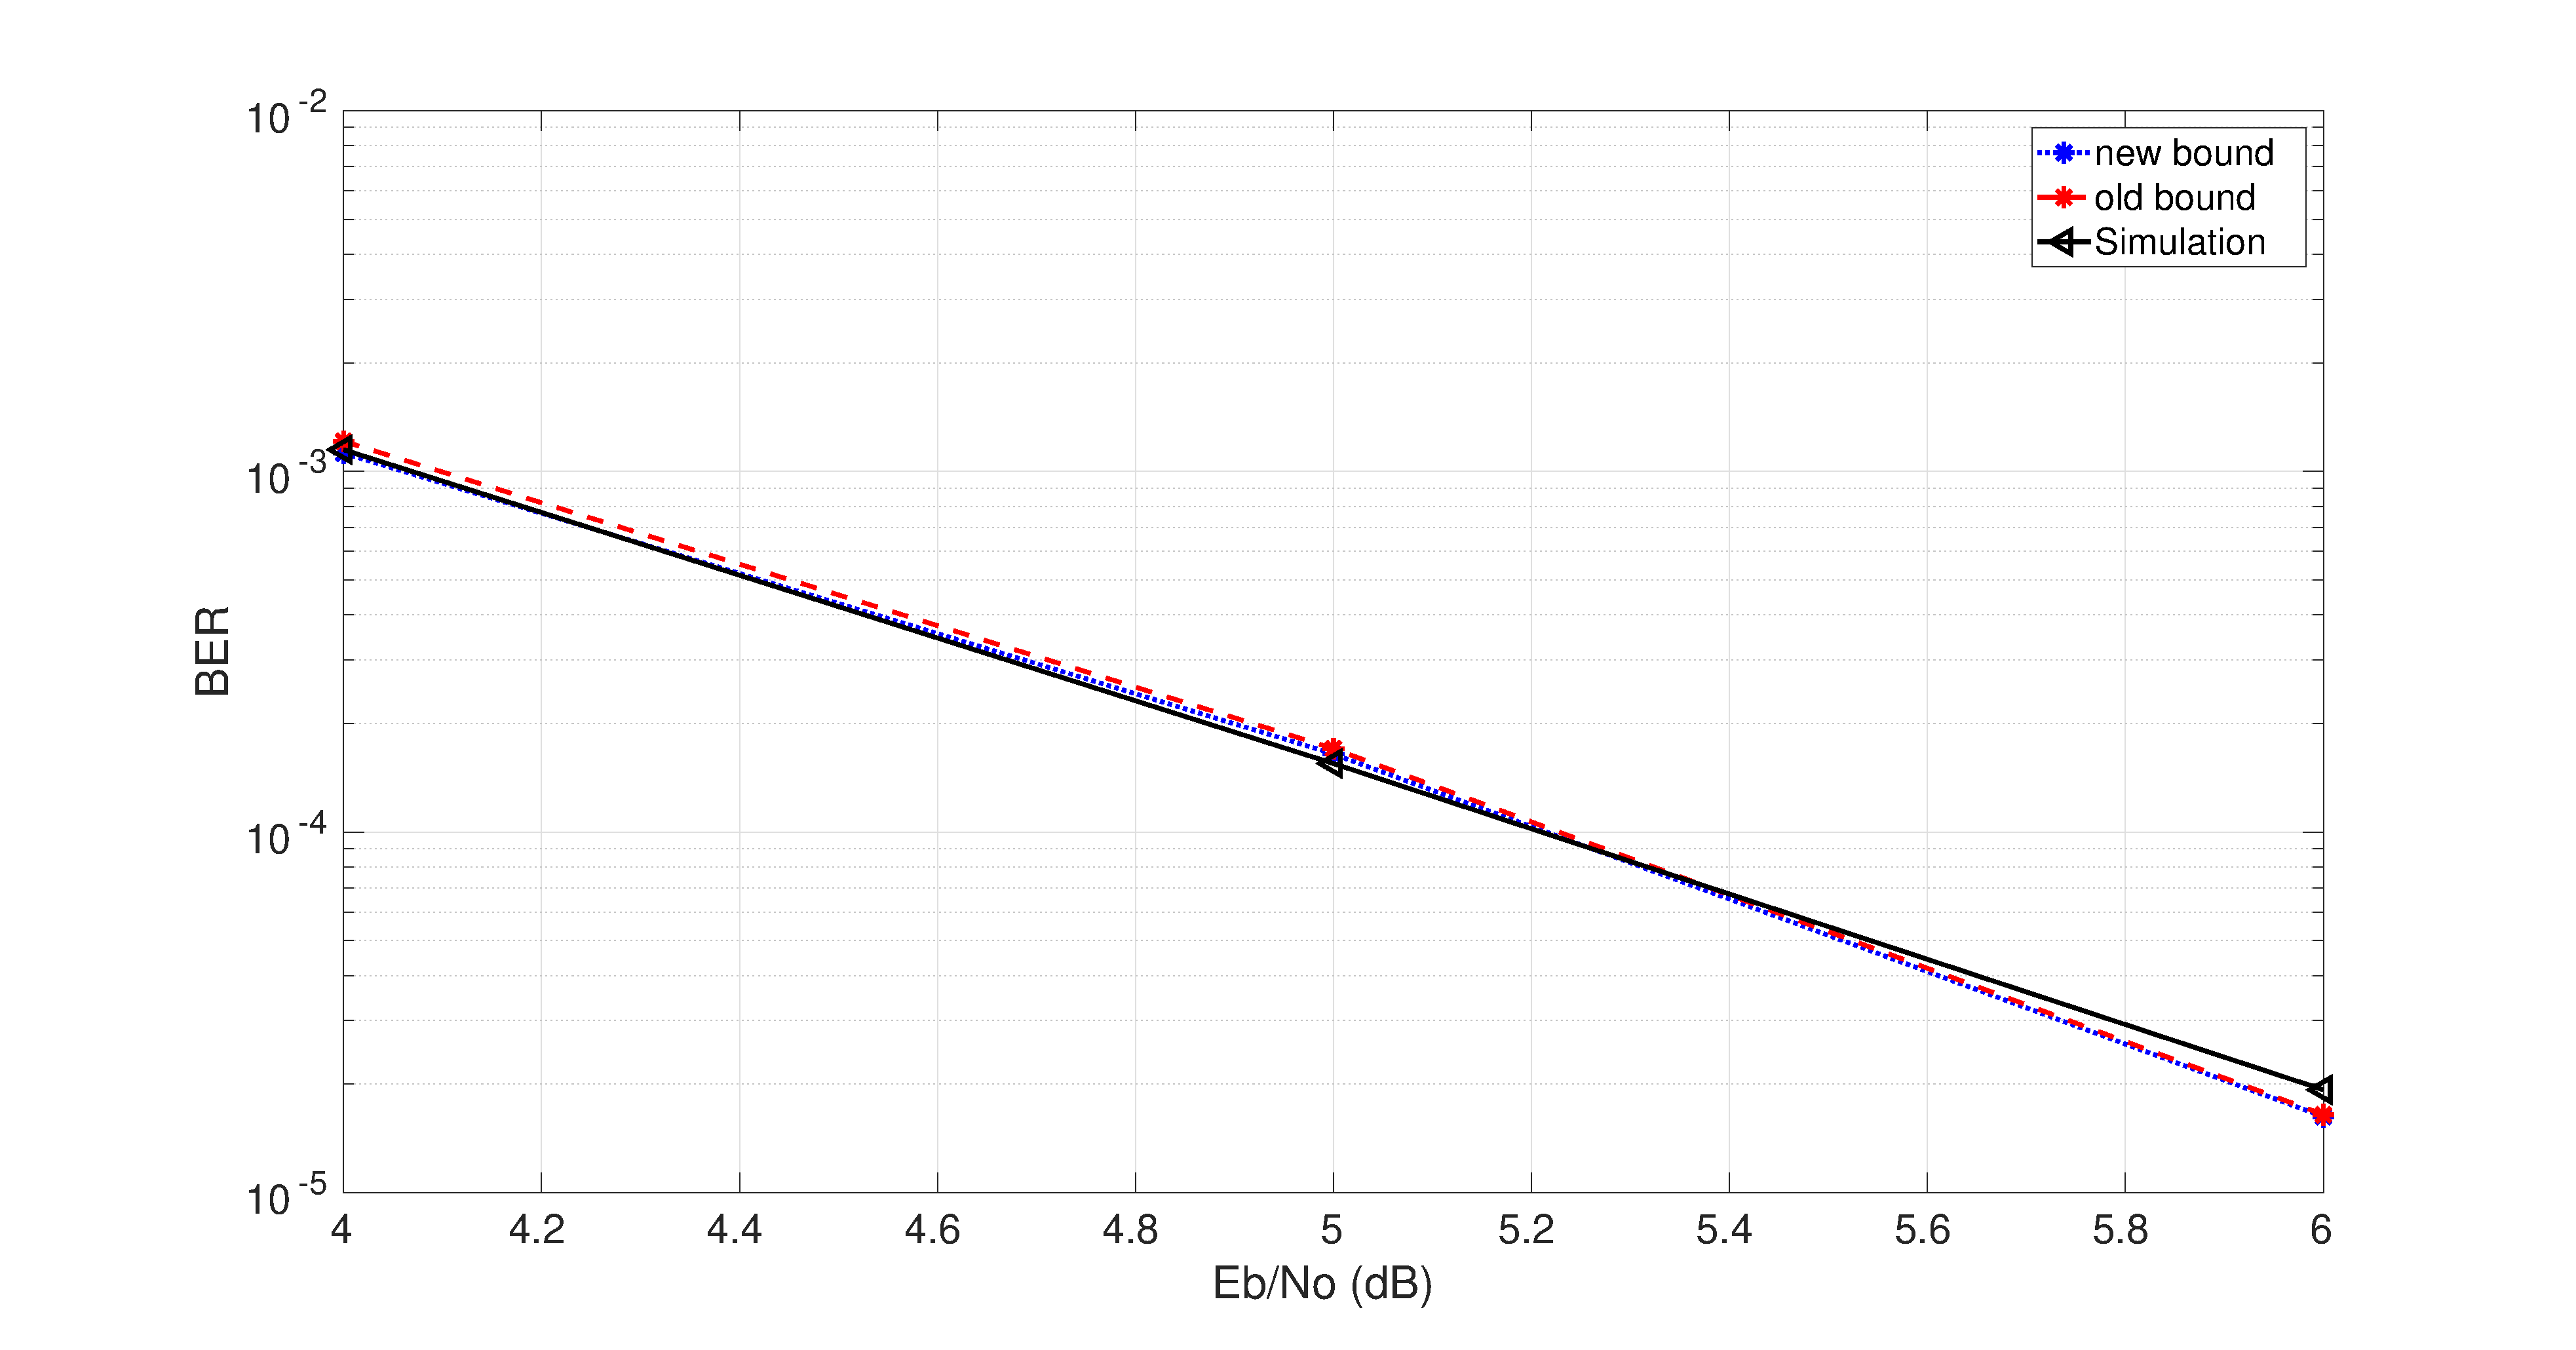
\includegraphics[width=0.5\textwidth]{./Images/RSC_5_7_v3.eps}
		\caption{Old Bound vs New Bound vs Simulation for 5/7 RSC Code}
		\label{simFig1}
		\end{figure}


\begin{figure}[h]
\centering
		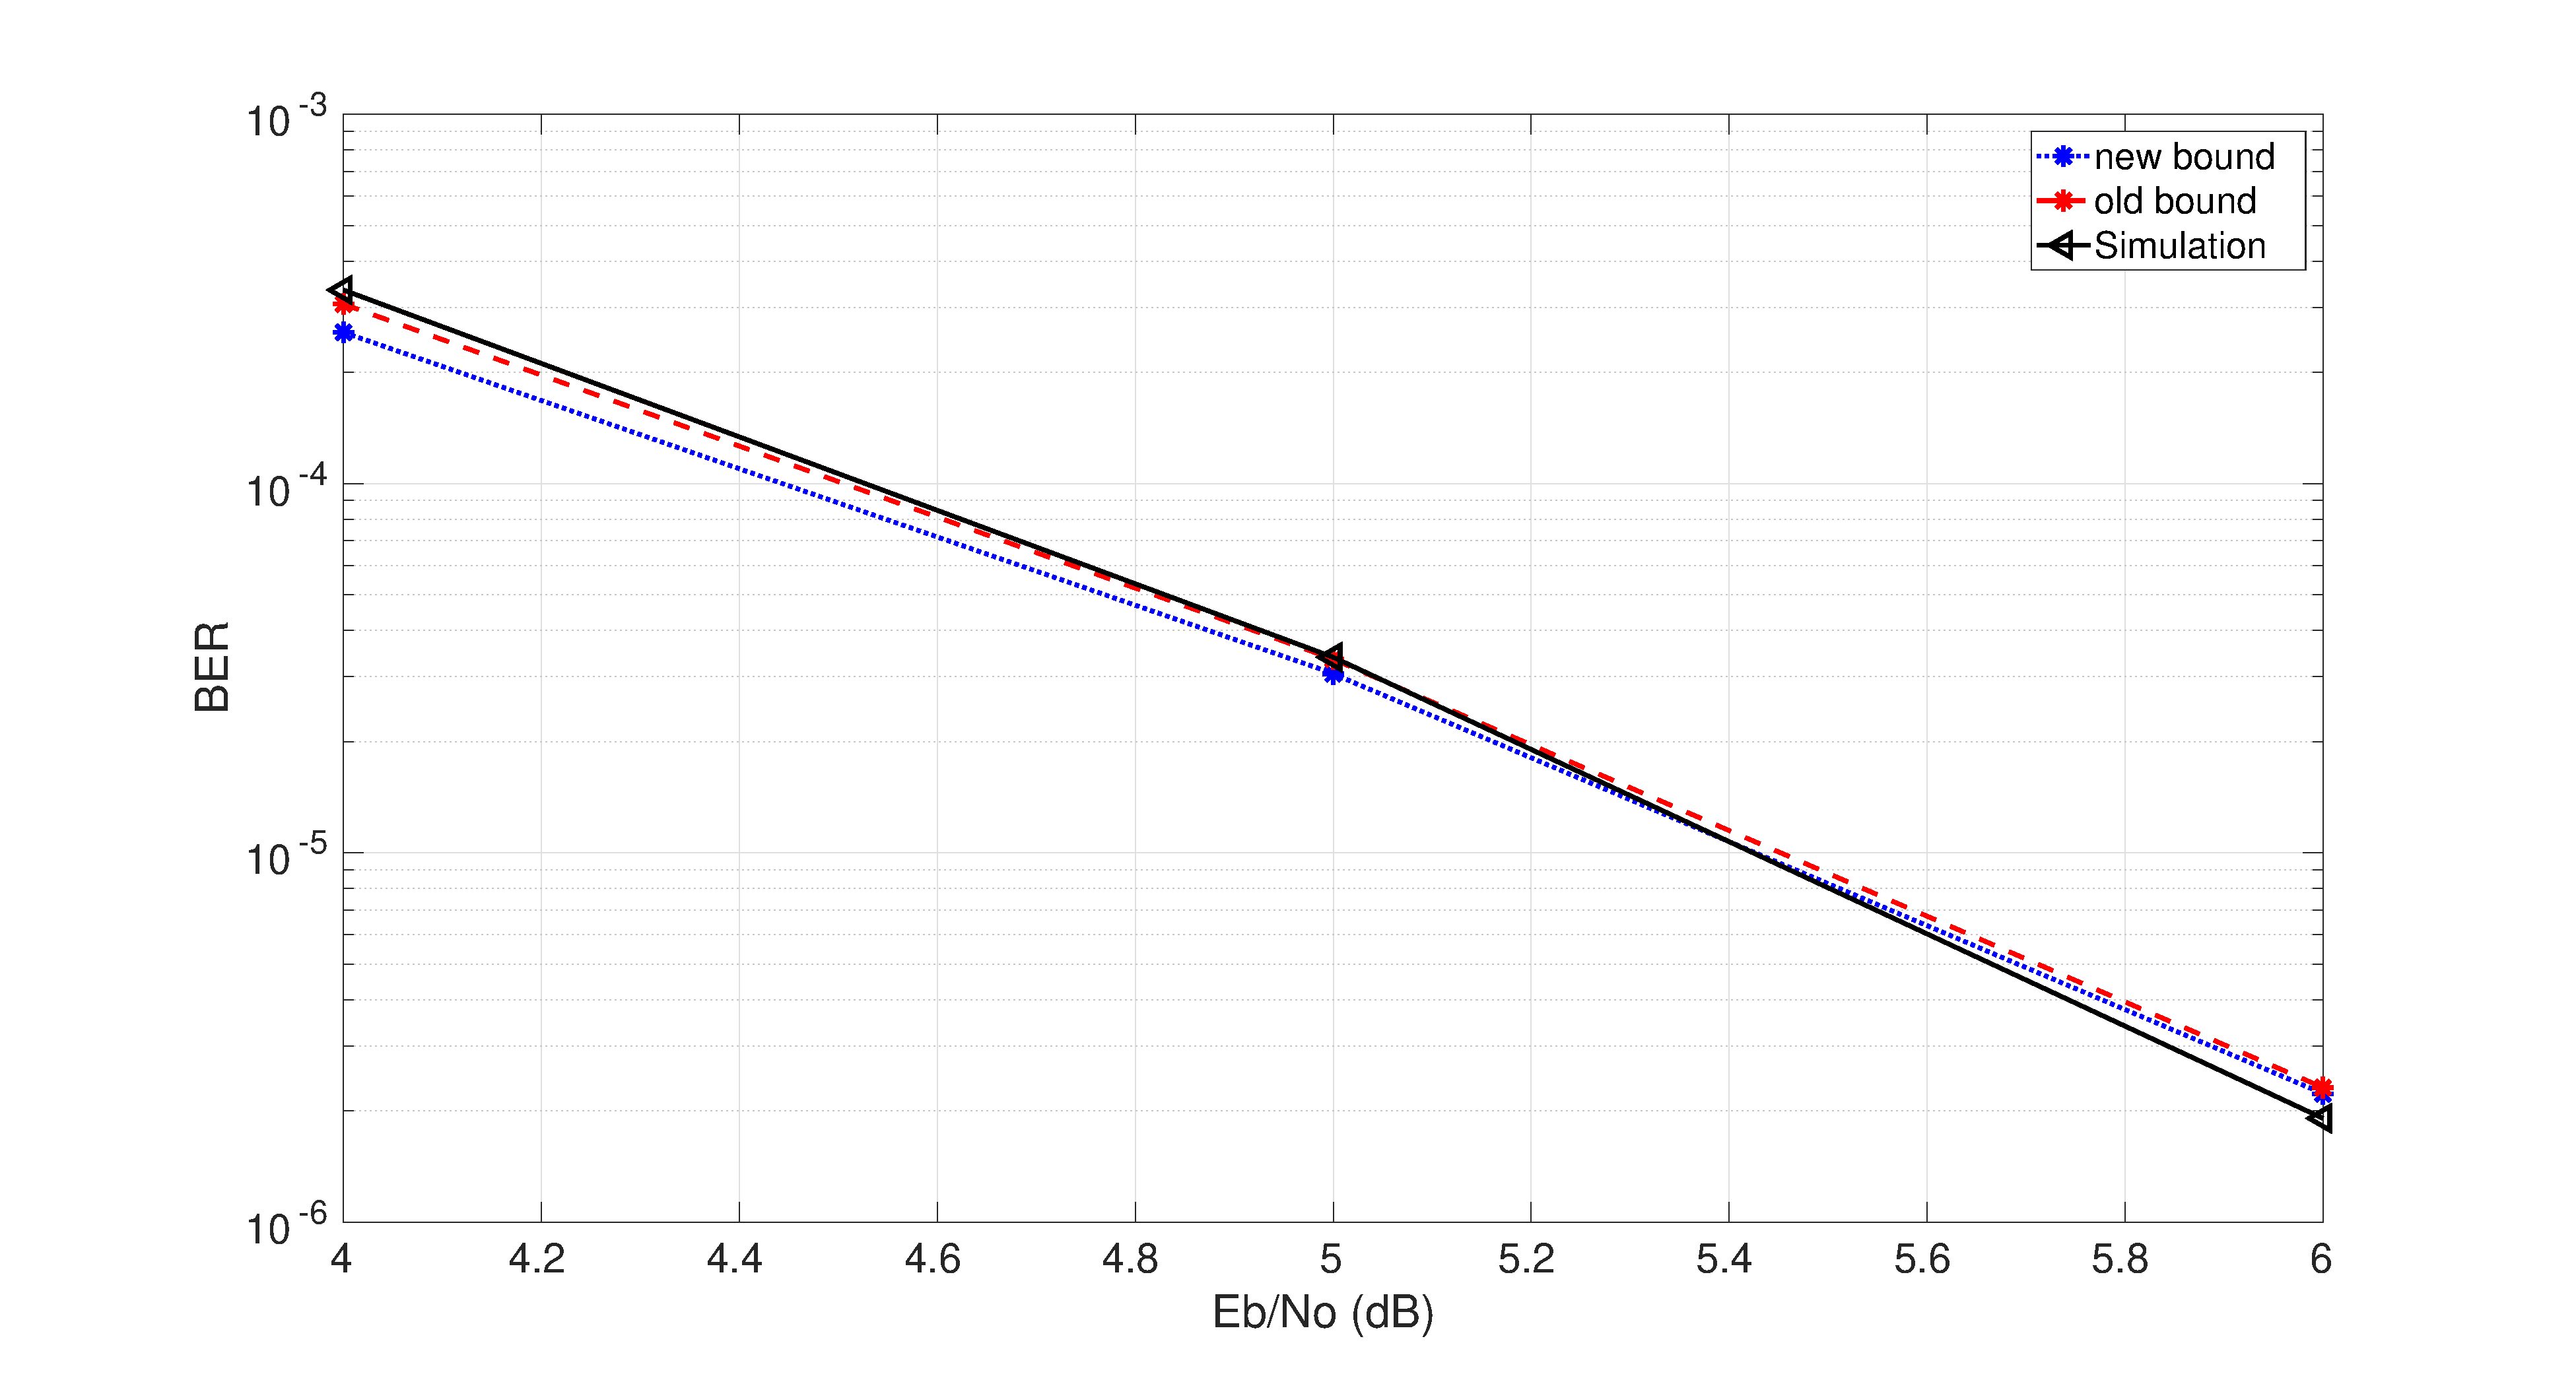
\includegraphics[width=0.5\textwidth]{./Images/RSC_37_21_v2.eps}
		\caption{Old Bound vs New Bound vs Simulation for 37/21 RSC Code}
		\label{simFig2}
		\end{figure}



